\chapter{Fyzikální veličiny}

Vlastnosti fyzikálních systémů (rozměry, hmotnost, náboj apod.) charakterizujeme kvantitativně pomocí fyzikálních veličin.

Fyzikální veličina $X$ má svou číselnou hodnotu (kvantitu) $\{X\}$ a jednotku $[X]$:
$$ X = \{X\}\,[X] $$
(často zkráceně značeno též $X = x\,[X]$).

Fyzikální zákony vyjadřují vztahy mezi fyzikálními veličinami pomocí matematických rovnic.

Podle toho, zda veličina závisí na velikosti systému (resp.~množství látky), dělíme veličiny na:
\begin{description}
    \item[intenzivní veličiny] nezávisejí na velikosti systému, jednotlivé části systému mají stejnou hodnotu jako celek (např.~teplota, hustota, tlak, koncentrace),
    \item[extenzivní veličiny] závisejí na velikosti systému, hodnota pro celý systém je rovna součtu hodnot jeho jednotlivých částí (např.~délka, hmotnost, objem, energie).
\end{description}

Veličiny můžeme také dělit podle jejich matematického charakteru (a chování při transformacích souřadnic):
\begin{description}
    \item[skalární veličiny] k~jejichž plnému určení stačí jediné číslo s~jednotkou (např.~hmotnost, čas, teplota),
    \item[vektorové veličiny] mají velikost a směr (ve trojrozměrném prostoru jsou určeny 3 složkami, v~relativitě 4 složkami), např.~poloha, rychlost, zrychlení, síla,
    \item[tenzorové veličiny] obecnější objekty (často reprezentované maticemi), které typicky popisují směrově závislou odezvu materiálu či anizotropní vlastnosti prostředí; typickým příkladem je tenzor deformace, tenzor mechanického napětí nebo tenzor setrvačnosti tuhého tělesa.
\end{description}

Speciálním případem jsou \emph{fyzikální pole}, což je přiřazení hodnoty veličiny (skalární, vektorové či tenzorové) každému bodu v~prostoru a v~čase (např.~gravitační či elektromagnetické pole), k~jejichž úplnému popisu je zapotřebí nekonečně mnoho hodnot (spojité stupně volnosti kontinua).

\section{Jednotky a rozměrová analýza}

Fyzikální veličiny mají jednotky. Standardně používanou soustavou jednotek je mezinárodní soustava \emph{SI}, která definuje 7 \emph{základních} jednotek:
\begin{center}
    \begin{tabular}{llcp{5.8cm}}
        \toprule
        Veličina & Základní jednotka & Značka & Princip definice (redefinice SI 2019) \\ \midrule
        délka & metr & m & fixací rychlosti světla $c$ a definice sekundy \\
        hmotnost & kilogram & kg & fixací Planckovy konstanty $h$ a definic s a m \\
        čas & sekunda & s & fixací frekvence cesiového přechodu $\Delta \nu_{\mathrm{Cs}}$ \\
        elektrický proud & ampér & A & fixací elementárního náboje $e$ a definice sekundy \\
        termodynamická teplota & kelvin & K & fixací Boltzmannovy konstanty $k_\mathrm{B}$ \\
        látkové množství & mol & mol & fixací Avogadrovy konstanty $N_\mathrm{A}$ \\
        svítivost & kandela & cd & fixací světelné účinnosti monochromatického záření \\
        \bottomrule
    \end{tabular}
\end{center}
ze kterých jsou další jednotky \emph{odvozeny}, např.~pro frekvenci $[f] = \unit{Hz} = \unit{s^{-1}}$, pro sílu $[F] = \unit{N} = \unit{kg.m.s^{-2}}$ nebo pro energii $[E] = \unit{J} = \unit{kg.m^2.s^{-2}}$. Soustava SI poskytuje také standardní \emph{předpony} (prefixy), které vyjadřují dekadické násobky a díly jednotek. V~současnosti jsou definovány:
\begin{center}
    \begin{tabular}{llc|llc}
        \toprule
        Předpona & Značka & Faktor & Předpona & Značka & Faktor \\ \midrule
        quetta & Q  & $10^{30}$ & deci   & d     & $10^{-1}$ \\
        ronna  & R  & $10^{27}$ & centi  & c     & $10^{-2}$ \\
        yotta  & Y  & $10^{24}$ & mili   & m     & $10^{-3}$ \\
        zetta  & Z  & $10^{21}$ & mikro  & $\mu$ & $10^{-6}$ \\
        exa    & E  & $10^{18}$ & nano   & n     & $10^{-9}$ \\
        peta   & P  & $10^{15}$ & piko   & p     & $10^{-12}$ \\
        tera   & T  & $10^{12}$ & femto  & f     & $10^{-15}$ \\
        giga   & G  & $10^{9}$  & atto   & a     & $10^{-18}$ \\
        mega   & M  & $10^{6}$  & zepto  & z     & $10^{-21}$ \\
        kilo   & k  & $10^{3}$  & jokto  & y     & $10^{-24}$ \\
        hekto  & h  & $10^{2}$  & ronto  & r     & $10^{-27}$ \\
        deka   & da & $10^{1}$  & kvekto & q     & $10^{-30}$ \\
        \bottomrule
    \end{tabular}
\end{center}
\begin{poznamka}
    Kilogram je jediná základní jednotka SI, která obsahuje předponu již ve svém základním názvu.
\end{poznamka}

Příroda (resp.~fundamentální fyzikální teorie) poskytuje tři základní rozměrové konstanty:
\begin{description}
    \item[Rychlost světla ve vakuu (definovaná, přesná)] $$c = \qty{299 792 458}{m/s}$$
    \item[Planckova konstanta (definovaná, přesná)] $$ h = \qty{6.62607015d-34}{J.s} $$ Často se používá \emph{redukovaná Planckova konstanta} $\hbar = h / (2\pi) \approx \qty{1.05457d-34}{J.s}$.
    \item[Newtonova gravitační konstanta] $$ G \approx \qty{6.6743d-11}{m^3.kg^{-1}.s^{-2}} $$
\end{description}

S~definicemi jednotek SI jsou dále pevně svázány tyto definující konstanty:
\begin{description}
    \item[Boltzmannova konstanta (přesná hodnota)] převod mezi termodynamickou teplotou a energií:
    $$ k_\mathrm{B} = \qty{1.380649d-23}{J.K^{-1}} $$
    \item[Avogadrova konstanta (přesná hodnota)] počet částic v~$1\ \unit{mol}$ látky:
    $$ N_\mathrm{A} = \qty{6.02214076d23}{mol^{-1}} $$
    \item[Elementární náboj (přesná hodnota)] definuje jednotku elektrického náboje coulomb ($\unit{C}$), pomocí níž a sekundy je definován ampér ($\unit{1}{A} = \unit{1}{C.s^{-1}}$):
    $$ e = \qty{1.602176634d-19}{C} $$
\end{description}

Mnoho oborů fyziky má zavedené vlastní jednotky vhodné pro studované škály délek, rychlostí či energií. Fundamentální konstanty navíc umožňují přirozený převod mezi zdánlivě nesouměřitelnými veličinami: například v~částicové fyzice je běžné udávat klidovou hmotnost v~jednotkách $\unit{eV}/c^2$ (při volbě přirozených jednotek $c=1$ přímo v~elektronvoltech $\unit{eV}$), kde $1\ \unit{eV} \approx \qty{1.602d-19}{J}$ je kinetická energie, kterou získá elektron urychlením potenciálovým rozdílem $1\ \unit{V}$. Ekvivalenci hmotnosti a energie vyjadřuje slavný Einsteinův vztah $E = mc^2$, odkud plyne $1\ \unit{eV}/c^2 \approx \qty{1.78d-36}{kg}$. Klidová hmotnost elektronu je potom $m_e \approx \qty{511}{keV}/c^2$ a hmotnost běžné octomilky ($m \approx \qty{1}{mg}$) činí řádově $m_{\mathrm{moucha}} \approx 10^{29}\ \unit{eV}/c^2$.

\begin{priklad}[Definice parseku]
    Jak změřit vzdálenost blízkých hvězd od Země? Změříme polohu hvězdy vůči vzdálenému hvězdnému pozadí (objektům na obloze tak dalekým, že se jejich zdánlivá poloha během roku nemění) ve dvou protilehlých bodech oběžné dráhy Země kolem Slunce. Z~toho získáme úhel $p$ (tzv.~roční paralaxu).

    \begin{center}
        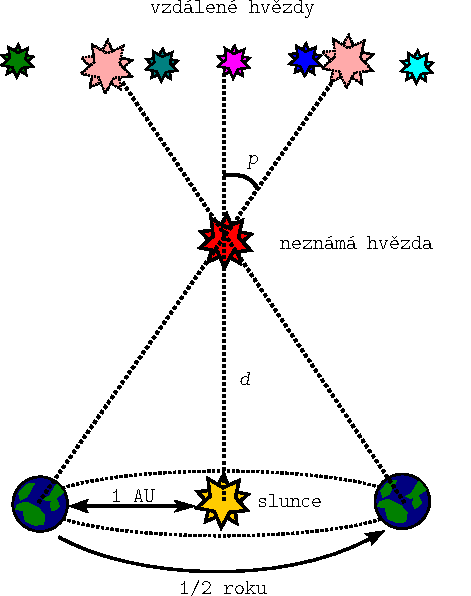
\includegraphics{chapters/figures/paralax.pdf}
    \end{center}

    Známe-li vzdálenost Země od Slunce, tj.~jednu astronomickou jednotku ($1\ \unit{au} \approx \qty{1.496d11}{m}$), je vzdálenost $d$ k~hvězdě rovna
    $$ d = \frac{\qty{1}{au}}{\tan p} \approx \frac{\qty{1}{au}}{p}, $$
    kde aproximace $\tan p \approx p$ platí pro malé úhly $p$ vyjádřené v~radiánech. Malé úhly se v~astronomii tradičně udávají v~úhlových minutách ($1' = (1/60)^\circ$) a v~úhlových vteřinách ($1'' = 1/60' = (1/3600)^\circ$).

    Jeden \emph{parsek} (pc, zkratka z~\emph{parallax of one second}) je definován jako vzdálenost, ze které vidíme úsečku o~délce $1\ \unit{au}$ kolmou k~paprsku vidění pod úhlem jedné úhlové vteřiny ($p = 1''$):
    $$ \qty{1}{pc} = \frac{\qty{1}{au}}{\tan(1'')} \approx \frac{\qty{1.496d11}{m}}{4{,}848 \times 10^{-6}} \approx \qty{3.086d16}{m} \approx \qty{3.26}{ly}, $$
    kde $\unit{ly}$ značí světelný rok (\emph{light-year}).
\end{priklad}

\subsection{Rozměrová analýza}

Fyzikální zákony jsou typicky vyjádřeny formou matematických rovnic spojujících fyzikální veličiny. Aby měly rovnice fyzikální smysl, musejí mít obě strany rovnice shodný rozměr (jednotku). Například pro Newtonův druhý zákon $F = ma$:
\begin{description}
    \item[Levá strana:] $$ [F] = \unit{N} = \unit{kg.m.s^{-2}} $$
    \item[Pravá strana:] $$ [m][a] = \unit{kg} \times \unit{m.s^{-2}} = \unit{kg.m.s^{-2}} $$
\end{description}
Tato nutná rozměrová homogenita nám poskytuje jednoduchý nástroj pro kontrolu, zda jsme se při výpočtu nedopustili algebraické chyby (rozměrová správnost je však nutnou, nikoli postačující podmínkou správnosti).

Ve fyzice hrají zásadní roli bezrozměrné veličiny a jejich skupiny. Až na triviální výjimky smějí být argumentem transcendentních matematických funkcí ($\sin$, $\cos$, $\exp$, $\ln$ apod.) výhradně bezrozměrné veličiny. To je patrné například z~Taylorova rozvoje funkce kosinus:
$$ \cos(x) = 1 - \frac{1}{2}x^2 + \frac{1}{24}x^4 - \dots $$
Aby měl součet na pravé straně fyzikální smysl, musejí mít všechny členy stejný rozměr jako číslo $1$, tj.~argument $x$ musí být bezrozměrný (např.~úhel v~radiánech).

Rozměrová analýza (formulovaná exaktně jako tzv.~\emph{Buckinghamův $\Pi$-teorém}) nám také umožňuje odhadnout tvar funkční závislosti mezi veličinami. Předpokládejme, že hledáme veličinu $Y$, která závisí na veličinách $X_1, X_2, \dots, X_n$. Pro mechanické veličiny vyjádřené v~základních jednotkách SI platí
$$ [X_k] = \unit{kg^{\alpha_k}.m^{\beta_k}.s^{\gamma_k}}, $$
a analogicky pro $[Y]$. Nejprve ze zadaných veličin sestavíme všechny nezávislé \emph{bezrozměrné kombinace} $\Pi_m$,
$$ \Pi_m = X_1^{b_1} X_2^{b_2} \cdots X_n^{b_n}, \quad [\Pi_m] = 1. $$
Lze-li sestrojit kombinaci veličin $X_k$ se stejným rozměrem jako $Y$, tedy $[Y] = [X_1^{a_1} X_2^{a_2} \dots X_n^{a_n}]$, pak lze hledaný vztah zapsat ve tvaru
$$ Y = C(\Pi_1, \Pi_2, \dots)\, X_1^{a_1} X_2^{a_2} \cdots X_n^{a_n}, $$
kde $C$ je neznámá funkce bezrozměrných parametrů $\Pi_m$. Pokud žádné nezávislé bezrozměrné parametry $\Pi_m$ neexistují, redukuje se $C$ na čistou číselnou konstantu (často řádu jednotek, případně násobek $2\pi$).

\begin{priklad}[Perioda kmitů kyvadla]
    S~jakou periodou $T$ kmitá matematické kyvadlo o~hmotnosti závaží $m$ a délce závěsu $l$ v~homogenním tíhovém poli s~tíhovým zrychlením $g$ při počáteční úhlové výchylce $\theta_0$?

    Rozměry jednotlivých veličin jsou:
    \begin{align*}
        [T] &= \unit{s},\\
        [m] &= \unit{kg},\\
        [l] &= \unit{m},\\
        [g] &= \unit{m.s^{-2}},\\
        [\theta_0] &= 1.
    \end{align*}
    Z~veličin $m, l, g$ nelze sestavit žádnou bezrozměrnou kombinaci (hmotnost $m$ se v~žádné další veličině nevyskytuje, proto musí mít nulový exponent, a sekundu v~$g$ lze kompenzovat pouze pomocí $l$, která sekundu neobsahuje). Jedinou bezrozměrnou veličinou je počáteční úhel $\theta_0$. Bezrozměrná funkce $C$ proto může záviset pouze na $\theta_0$.

    Rozměr sekundy z~veličin $m, l, g$ získáme jediným možným způsobem:
    $$ T \sim m^0 l^{1/2} g^{-1/2} = \sqrt{\frac{l}{g}}. $$
    Celkový vztah má tedy tvar $T = C(\theta_0) \sqrt{l/g}$.
    Přesné řešení pohybových rovnic pro \emph{malé kmity} dává $C(0) = 2\pi$, tedy
    $$ T = 2\pi\sqrt{\frac{l}{g}}. $$
    Při velkých výchylkách závisí perioda na $\theta_0$ (přesné řešení vede na úplný eliptický integrál prvního druhu).
\end{priklad}

\begin{priklad}[Explozivní energie jaderné bomby]\footnote{S~tímto řešením přišel v~roce 1950 britský fyzik G.~I.~Taylor; převzato z~knihy \emph{Classical Mechanics}, David Tong, Cambridge University.}
    V~roce 1945 byla v~Novém Mexiku provedena první jaderná zkouška s~kódovým označením Trinity. Z~tohoto testu byla později odtajněna a zveřejněna série fotografií, z~nichž bylo možné vyčíst poloměr rázové vlny v~různých časových okamžicích po detonaci. Níže uvedený snímek zachycuje rázovou vlnu o~poloměru $R \approx \qty{150}{m}$ v~čase $t = \qty{0.025}{s}$. Jak velká energie $E$ byla při výbuchu uvolněna?
    \begin{center}
        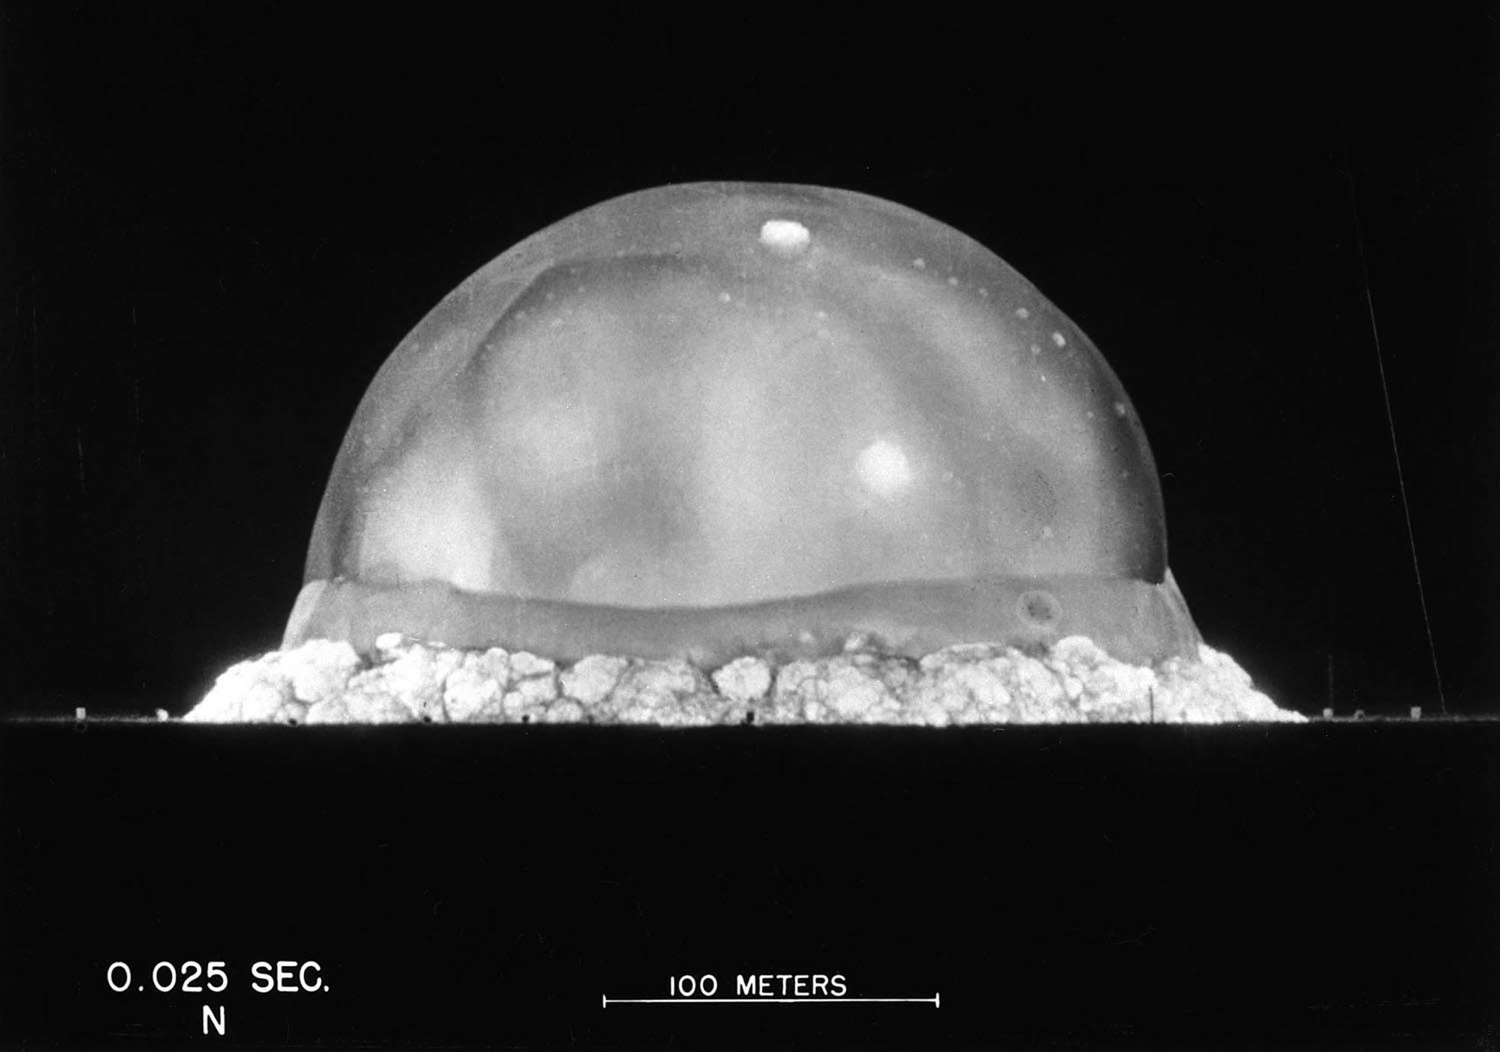
\includegraphics[width=0.5\textwidth]{chapters/figures/trinity_fireball.jpg}
    \end{center}

    Samotná jaderná řetězová reakce trvá extrémně krátce, takže v~okamžiku zachycení snímku již byla veškerá energie uvolněna a soustředěna v~expandující ohnivé kouli. Na čem může šíření této silné rázové vlny záviset? Uvažujme veličiny popisující stav: počáteční tlak $p_0$ a hustotu $\rho_0$ okolního vzduchu, tlak $p$ a hustotu $\rho$ plynu uvnitř ohnivé koule a konečně poloměr čela rázové vlny $R$ v~čase $t$. Rozměry těchto veličin jsou $[p] = [p_0] = \unit{kg.m^{-1}.s^{-2}}$, $[\rho] = [\rho_0] = \unit{kg.m^{-3}}$, $[R] = \unit{m}$ a $[t] = \unit{s}$.

    Z~těchto veličin lze sestavit tři nezávislé bezrozměrné kombinace:
    $$ \Pi_1 = \frac{p_0}{p}, \quad \Pi_2 = \frac{\rho}{\rho_0}, \quad \Pi_3 = \frac{p_0 t^2}{\rho_0 R^2}. $$
    Uvnitř ohnivé koule panuje obrovský tlak ($p \gg p_0$) a plyn je extrémně zahřátý a zředěný, proto $\Pi_1 \ll 1$ a $\Pi_2 \ll 1$. Pro třetí bezrozměrnou kombinaci si všimněme, že $p_0 / \rho_0 \approx c_{\mathrm{zvuk}}^2$, kde $c_{\mathrm{zvuk}} \approx \qty{340}{m/s}$ je rychlost zvuku v~okolním vzduchu. Ze snímku plyne $t^2 / R^2 \approx (0{,}025)^2 / 150^2 \approx \qty{2.8d-8}{s^2.m^{-2}}$, takže
    $$ \Pi_3 \approx c_{\mathrm{zvuk}}^2 \frac{t^2}{R^2} \approx (\qty{340}{m/s})^2 \times (\qty{2.8d-8}{s^2.m^{-2}}) \approx 3 \times 10^{-3} \ll 1. $$
    Protože jsou všechny tyto parametry zanedbatelné vůči jedničce, šíření silné rázové vlny prakticky nezávisí na tlacích $p$ a $p_0$ ani na vnitřní hustotě $\rho$. Jedinými relevantními parametry zůstávají počáteční hustota okolního vzduchu $\rho_0$, poloměr $R$ a čas $t$.

    Rozměr energie je $[E] = \unit{kg.m^2.s^{-2}}$. Jediný způsob, jak z~veličin $\rho_0$, $R$ a $t$ sestavit rozměr energie, je
    $$ E = C \frac{\rho_0 R^5}{t^2}, $$
    kde bezrozměrný koeficient $C$ může obecně záviset pouze na $\Pi_k \ll 1$, lze jej tedy s~vysokou přesností považovat za univerzální konstantu. Rozměrová analýza samotnou hodnotu $C$ určit neumí, avšak z~hydrodynamické teorie silných rázových vln plyne pro vzduch s~adiabatickým exponentem $\gamma = 1{,}4$, že $C \approx 1{,}03 \approx 1$.

    Dosazením hodnot pro vzduch ($\rho_0 \approx \qty{1.3}{kg/m^3}$) dostáváme:
    $$ E \approx 1 \times \frac{\qty{1.3}{kg/m^3} \times (\qty{150}{m})^5}{(\qty{0.025}{s})^2} \approx \qty{1.6d14}{J}. $$
    Jedna kilotona TNT ($1\ \unit{kt\ TNT}$) odpovídá uvolnění přibližně $\qty{4.184d12}{J}$. Odhad energie výbuchu je tedy
    $$ E \approx \qty{38}{kt\ TNT}. $$
    Skutečná uvolněná energie testu Trinity činila přibližně $\qty{20}{kt\ TNT}$ až $\qty{22}{kt\ TNT}$ (rozdíl je způsoben zjednodušeným odečtem poloměru a tím, že část energie byla vyzářena v~podobě tepelného a ionizujícího záření). Na pouhý odhad z~rozměrové analýzy a jediné fotografie jde o~mimořádně dobrý výsledek.
\end{priklad}


